\documentclass{jflart}
\usepackage[utf8]{inputenc}
\usepackage[T1]{fontenc}

% Numéro et année des JFLAs visées par l'article, obligatoire.
\jfla{37}{2027}

\usepackage{lmodern}
\usepackage{enumitem}
\usepackage{amsmath,amssymb}
\usepackage{geometry}
\usepackage{graphicx}
\usepackage{xcolor}
\usepackage{listings}
\usepackage{hyperref}
\usepackage{tikz-cd}
\usetikzlibrary{arrows.meta, positioning, calc}

\lstdefinelanguage{Rocq}{
  morekeywords={Fixpoint,match,with,end,fun,let,in,Theorem,
    Lemma,Proof,Qed,Definition,forall,exists},
  sensitive=true,
  morecomment=[s]{(*}{*)},
  morestring=[b]"
}
\geometry{margin=1in}
\setlist[itemize]{leftmargin=*}
\lstset{numbers=left,basicstyle=\small\ttfamily, columns=fullflexible,keepspaces=true, frame=single, breaklines=true, backgroundcolor=\color{gray!7}}

\title{Improving the Tactics \texttt{ring} and \texttt{field}\\
 }
\author[1]{Thomas Portet}
\author[2]{Yves Bertot}
\affil[1]{Université Côte d'Azur, INRIA Sophia Antipolis, France}
\affil[2]{INRIA Sophia Antipolis, France}
\begin{document}
\maketitle

\begin{abstract}
This paper describes an extension of Rocq's \cite{rocq-prover} reflexive algebraic tactics. The main goal is to make \texttt{ring} and \texttt{field} usable on expressions that
contain functions outside the ring or field fragment. The approach rewrites the
arguments of such functions, computes polynomial greatest common divisors with
an OCaml oracle, and exposes the result to Rocq through ELPI foreign calls.
\end{abstract}
\section{Motivation}

We would like to formalize undergraduate mathematics in a style that remains close to ordinary pen-and-paper reasoning, while retaining the formal guarantees of a proof assistant. We therefore choose to work in a simple ambient theory, with a small collection of familiar mathematical objects and operations, and to allow users to express mathematical arguments through high-level declarative steps rather than low-level proof-assistant transformations.
\newline \newline
This setting motivates the question of how algebraic automation should behave when an algebraic expression occurs inside a function that is not itself part of the algebraic theory handled by the tactic. For example, a student should ideally be able to write

\[
\log(\pi^2+\pi\times\pi)=\log(2\pi^2)
\]
without having to explicitly expose the intermediate algebraic rewriting
\[
\pi^2+\pi\times\pi=2\pi^2.
\]
The proof assistant should be able to recognize and justify this transformation automatically.\newline
The difficulty is that the outer function $\log$ is not a ring operation. Consequently, the algebraic tactic cannot treat the whole expression as a ring expression.

The existing \texttt{ring\_simplify} tactic addresses this issue for ring expressions by recursively simplifying algebraic expressions inside function applications.
% TODO: Here, the analogous example with log(\frac{2 \pi}{4}) = log (\frac(3 \pi}{6}) devrait être donné, en expliquant que field_simplify does not help as much as ring_simplify does in the other case
However, the analogous approach does not directly extend to field expressions. This raises the question of how to obtain a suitable representation of field expressions when they occur inside functions that the field normalizer does not handle.
\section{Reflexive Algebraic Normalization}
The starting point is the way Rocq's reflexive algebraic tactics normally solve
equalities. Rather than applying a sequence of rewriting lemmas, the tactic
reifies the input expression into an internal representation of the relevant
algebraic structure, computes its normal form, and uses this computation to
construct a proof. This approach is exemplified by the reflective ring tactic of Grégoire and Mahboubi \cite{gregoire2005proving}.


\subsection{Ring normalization}

The \texttt{ring} tactic works with integer constants, addition, multiplication, subtraction, and variables. Expressions outside this language are treated as fresh variables during reification. Thus, for an expression such as

$$
  \pi^2+\pi\mathbin{\times}\pi,
$$

the constant $\pi$ can be represented by a fresh variable $X$. The tactic then normalizes the resulting polynomial expression. When the normalized expression is reconstructed as a Rocq term, the fresh variable $X$ is replaced by the original expression $\pi$.

More generally, the process can be described in three steps:
\begin{enumerate}
\item reify the input expression, replacing supported operations by constructors in an internal polynomial representation and treating unsupported expressions as fresh variables;
\item normalize the resulting polynomial by collecting coefficients and combining like monomials;
\item conclude when the normalized expressions are syntactically equal.
\end{enumerate}


Although the arguments of the two logarithms are polynomial expressions, the complete terms

$$
  \log(\pi^2+\pi\mathbin{\times}\pi)
  \qquad\text{and}\qquad
  \log(2\pi^2)
$$

are themselves outside the polynomial language. At the level at which \texttt{ring} sees them, they therefore become distinct atoms. The tactic cannot discover that these atoms are equal by simplifying their arguments.

\subsection{Deep ring simplification}\label{sec:deep-ring}

The natural way to address this limitation is to apply ring simplification recursively inside function applications. Instead of treating an entire unrecognized function application as an indivisible atom, we first simplify the expressions occurring in its arguments and then reconsider the enclosing expression.

For example,

$$
  \cos(x+\cos(x+x))
  =
  \cos(\cos(2x)+(1-(1-x))).
$$

The relevant subexpressions include

$$
  x+\cos(x+x),\qquad
  x+x,\qquad
  \cos(2x)+(1-(1-x)),
  \qquad\text{and}\qquad
  2x.
$$

The inner expression $x+x$ can first be normalized to $2x$. The enclosing expression can then be reified again, with $\cos(2x)$ as an atom, allowing

$$
  \cos(2x)+(1-(1-x))
$$

to be normalized to

$$
  x+\cos(2x).
$$

The original equality consequently reduces to

$$
  \cos(x+\cos(2x))
  =
  \cos(x+\cos(2x)).
$$

This gives a natural recursive strategy for expressions containing unrecognized
functions: simplify their arguments, rebuild the function applications from
the simplified arguments, and continue at enclosing levels.

The same idea applies to the motivating logarithm example. The argument

$$
  \pi^2+\pi\mathbin{\times}\pi
$$

can be normalized to $2\pi^2$ before the surrounding $\log$ application is considered. The two sides then contain the same function application, so the outer equality can be closed.

This approach works naturally for \texttt{ring} because polynomial normalization provides a canonical representation of the algebraic expression. 
The recursive strategy described above is implemented by calling
\texttt{ring\_simplify}, which takes a list of expressions and
normalizes them, even inside function applications.


One implementation issue arose when reusing \texttt{ring\_simplify}: successive recursive calls could oscillate between two expressions. For instance, one call could rewrite (x+y) as (y+x), while the next would rewrite it back to (x+y). To prevent this, we first collect all variables occurring in the expression and then call \texttt{ring\_simplify} with these variables as explicit arguments, followed by the expressions to normalize. This ensures that recursive calls use a consistent set of variables and prevents such oscillations. 

\section{The limits of \texttt{field\_simplify}}
An analogous approach does not work for \texttt{field\_simplify}, which does not produce a canonical representation of the input expression. 
Consider
\[
  \frac{\pi}{\pi^2+\pi^2}=\frac{1}{2\pi}.
\]
The \texttt{field} tactic can prove this if it proves $\pi^2+\pi^2\ne0$ and
$\pi\ne0$.
In practice, \texttt{field} reduces the equality to these non-zero side conditions; they still have to be proven separately, for example using the positivity of
$\pi$.
Now consider the variant
\[
  \log\!\left(\frac{\pi}{\pi^2+\pi^2}\right)
  = \log\!\left(\frac{1}{2\pi}\right).
\]
Here \texttt{field} fails because $x\mapsto\log(x)$ is not a field
expression. The same issue occurs for any outer function that is not handled by the tactic, such as $\exp$, $\sin$, or $\cos$.


The standard \texttt{field} tactic represents expressions as fractions, but it compares those fractions by cross multiplication:
\[
  q\ne0\ \land\ s\ne0
  \quad\Longrightarrow\quad
  \left(\frac{p}{q}=\frac{r}{s}
  \quad\Longleftrightarrow\quad
  p\times s=q\times r\right).
\]
This means a fraction does not need to be reduced in order to prove an equality.
For example, $3\pi/6=2\pi/4$ is established by checking the cross-product
identity $3\pi\times4=6\times2\pi$ together with the non-zero conditions on the
denominators.
The difficulty is subtler when the fraction occurs inside a function. The
tactic can prove that

$$
  \frac{3\pi}{6}=\frac{2\pi}{4}
$$

by cross multiplication, but this proof does not require either fraction to
be rewritten to a common representative. In particular, the two sides can
remain syntactically different after the \texttt{field\_simplify} calls.

%TODO this example should be in the motivation section
This distinction does not matter when the equality of the two fractions is
the final goal. Once the cross-product equality and the required non-zero
conditions have been established, the proof is complete. It matters when the
fraction occurs as an argument of a function that is unrecognized by the field
normalizer. Consider

$$
  \cos\left(\frac{3\pi}{6}\right)
  =
  \cos\left(\frac{2\pi}{4}\right).
$$

The field normalizer can reason about the two fractions, but it does not
normalize the surrounding occurrences of \texttt{cos}. The two function
applications can therefore contain different terms even when their
arguments could be proved equal.

The required operation is consequently stronger than proving equality of
the two fractions. We need to transform both fractions to a common
representative that can be used in the surrounding expression. For the
example above, a suitable representative is $ \frac{\pi}{2}$.


The desired transformation is therefore

$$
  \cos\left(\frac{3\pi}{6}\right)
  \longrightarrow
  \cos\left(\frac{\pi}{2}\right)
  \longleftarrow
  \cos\left(\frac{2\pi}{4}\right).
$$
A polynomial gcd provides the missing operation. Given a numerator \(N\) and denominator \(D\), we compute a common factor \(\gamma\) and the corresponding quotients \(\nu\) and \(\delta\). This yields a reduced representation of the fraction that can be propagated through an enclosing function application.


\section{Making room for an oracle}
The existing theorem that justifies the \texttt{field\_simplify} tactic has the
following shape:
\[
 \operatorname{Fnorm} e = r \Longrightarrow
 \operatorname{FEeval}(l,e)=
 \frac{\operatorname{Pphi\_pow}(l,\operatorname{norm}(\operatorname{num}(r)))}
  {\operatorname{Pphi\_pow}(l,\operatorname{norm}(\operatorname{den}(r)))}.
\]
Starting from an arbitrary expression in the studied field, for instance \(\frac{1}{\pi} + \frac{1}{\cos(1)}\), the reification produces the expression
\(e = \frac{1}{X_0} + \frac{1}{X_1}\) and the list of bindings \([\pi;\cos(1)]\),
so that \(FEeval(l, e)\) computes to the initial expression 
\(\frac{1}{\pi} + \frac{1}{\cos(1)}\).  The function \(\operatorname{Fnorm}\) is a gallina-language function that computes a fraction of ring expressions, together with a collection of expressions that should all be non zero.  The name \(\operatorname{Fnorm}\) is poorly chosen, because this function does not compute a normal form, it only ensures that the expression now has the shape of a single fraction whose numerator and denominator are both ring expressions (of the kind to be processed by the ring machinery).  The ring expressions are themselves not guaranteed to be in normal form.

In the case of the input expression \(e = \frac{1}{X_0} + \frac{1}{X_1}\), \(r\) has the shape \(r = \frac{X_1 + X_0}{X_0 X_1}\), together with the conditions that \(\pi\) and \(\cos(1)\) should not be 0.

The next step of processing the formula is to compute the ring normal forms of both parts of the fraction. This is performed by the calls to the \(norm\)
function that appear in the right-hand side of the conclusion equality.

The shape of this theorem states clearly that the numerator and the
denominator are processed independently.  If there is a common factor,
it is not removed by the calls to \(\operatorname{norm}\).

\label{sec:extension-lemma}
In our extension to the \texttt{field\_simplify} tactic, we instead rely on a
theorem with the following shape:

\[
\begin{array}{l}
 \operatorname{Fnorm} e = r \Longrightarrow\\
  \forall m~\nu~\delta~\gamma,\\
  m \neq 0 \\

  m \times \operatorname{norm}(\operatorname{num}(r)) = \nu\gamma \Longrightarrow\\
  m \times \operatorname{norm}(\operatorname{den}(r))= \delta\gamma \Longrightarrow\\
  \operatorname{FEeval}(l,e)=
  \frac{\displaystyle{\operatorname{Pphi\_pow}(l, \nu)}}
       {\displaystyle{\operatorname{Pphi\_pow}(l, \delta)}}.
\end{array}
\]

In what follows, we name \(N\) and \(D\) the numerator
\(\operatorname{norm}(\operatorname{num}(r))\) and the denominator \break
\(\operatorname{norm}(\operatorname{den}(r))\), respectively.  In this theorem, \(m\)
is an integer, and \(\nu\), \(\delta\), and \(\gamma\) are polynomials
in normal form.  This theorem is a direct consequence of the previous one, but it allows the ultimately produced fraction to be cleaned of common polynomial factors,
if these factors are included in the \(\gamma\) polynomial.

The four values \(m\), \(\nu\), \(\delta\), and \(\gamma\) have to be produced for
this theorem to be applied, and this is where an external
computation, which we will call an oracle in the rest of this paper, is needed.

In practice, we rely on an implementation of a Gröbner basis algorithm to
compute the greatest common divisor of the two polynomials.  This algorithm
operates on polynomials with rational coefficients.  It is easy to translate
our polynomials \(N\) and \(D\), which have integer coefficients, into polynomials
with rational coefficients, but when processing the result of the greatest
common divisor computation, we need to recover polynomials with integer
coefficients.  This is where the integer \(m\) is needed.  If we have candidate
polynomials \(\nu'\), \(\delta'\), \(\gamma'\) with rational coefficients, we only need to find two numbers
\(m_1\) and \(m_2\), so that \(m_1 \times \nu' = \nu\) has integer coefficients, and
so do \(m_1 \times \delta' = \delta \) and \(m_2 \times \gamma' = \gamma\), in this
case \(m=m_1 m_2\).

\subsection{A complete example}

The following example illustrates a computation where we take advantage of
the gcd computation.  Consider
\[
\frac{4 X^2-1}{2X^2+5X+2},
\]

The numerator and denominator are

\[
  N=4X^2-1,\qquad D=2X^2+5X+2.
\]

The polynomial gcd computation returns

\[
  m = 8,
  \qquad
  \gamma=16X+8,
  \qquad
  \nu=2X-1,
  \qquad
  \delta=X+2.
\]

These values satisfy the following equalities
\begin{equation}
  mN=\nu\gamma,
  \qquad
  mD=\delta\gamma.
  \label{eq:factorization-identities}
\end{equation}

In this example the scale factor is $m=8$.

The fraction can consequently be represented as
\[
  \frac{N}{D}
  =
  \frac{\nu}{\delta}
  =
  \frac{2X-1}{X+2}.
\]
The gcd computation provides a reduced representation of the fraction that
can be used to rewrite the argument of \(f\). In particular, the original
function application can be rewritten as

\[
f\left(\frac{4 X^2-1}{2X^2+5X+2}\right)
\longrightarrow
f\left(\frac{2X-1}{X+2}\right).
\]

The rewrite is justified by the factorization identities ~\ref{eq:factorization-identities} verified by Rocq.

\subsection{Implementation of the oracle}
The oracle is implemented as an OCaml program, which operates on sequences of
monomials to represent multivariate polynomials with rational coefficients.
The data type used in the program has the following shape:
\begin{lstlisting}[language=ML]
type monomial = { coef: rat; exps: (int * int) list }
type mpoly = monomial list
\end{lstlisting}
A monomial
consists of a rational coefficient and a sorted list of pairs $(i,e)$, where
$i$ is a variable index and $e$ is its exponent:


For example, the monomial

$$
  3X_1^2X_4
$$

is represented by the coefficient $3$ and the exponent list

$$
  [(1,2);(4,1)].
$$
Polynomial arithmetic, monomial ordering, reduction, and Buchberger's
algorithm operate on this sparse representation. Rational coefficients
are used because the polynomial computations sometimes use division
and can introduce non-integral coefficients. Monomials are ordered
lexicographically, with lower variable indices taking precedence. This order
determines the leading monomial used in polynomial reduction and
Buchberger's algorithm.

To facilitate the communication with Rocq's implementation of polynomials, we
chose to implement an OCaml datatype of ring expressions based only on integer constants, variables, addition and
multiplication.  The datatype description has the following shape:
\begin{lstlisting}[language=ML]
type poly =
| Const of int | Var of int | Add of poly * poly | Mul of poly * poly
\end{lstlisting}
This datatype is isomorphic to a subset of the datatype \texttt{PExpr} used in
the implementation of the ring tactic.
Before performing polynomial computations, the implementation converts an
input expression of type \texttt{poly}
to type \texttt{mpoly}.  After computations, results are converted back
to \texttt{poly}.

We use Gröbner basis computations because it is well known that the
least common multiplier of two polynomials \(p\) and \(q\) appears naturally
in the Gröbner basis generated for the family \((1 - X_0) p, X_0 q\), if \(X_0\)
is not used in \(p\) nor in \(q\) and this variable is smaller than all others in the
order used for the computation.  Once the least common multiplier is obtained,
it is easy to derive the greatest common divisor.

\section{The Rocq--ELPI--OCaml interface}
\subsection{Experimental setup}
To work at an early experimental stage, we chose a design that re-uses as
much as possible the current implementation of the \texttt{ring}-like
tactics but avoids modifying
any part of the Rocq main program.  As a result, our experiment
currently works with an unmodified version of the \texttt{rocq-core}
package, but a modified version of the \texttt{rocq-stdlib} package.

The code in \texttt{rocq-core} assumes that all behavior of the \texttt{ring}-like tactics is governed by 4 lemmas, each of which is an
instantiation of a generic lemma parameterized by arbitrary ring or
field structures.  In our case, we need to use the extra lemma presented in
Section~\ref{sec:extension-lemma} that
accounts for the possibility of calling an oracle after the
reification step.  We added such a lemma in the \texttt{rocq-stdlib}
package, under the name \texttt{Field\_rw\_pow\_correct\_w\_gcd}, its
statement is a modification of the existing \texttt{Field\_rw\_pow\_correct}, which is used by the existing
\texttt{field\_simplify} tactic.

We then created tactics to harness the extra lemma and the oracle.
Ultimately all these tactics should belong in the \texttt{rocq-stdlib}
package, but since recompiling the \texttt{stdlib} package takes about 50
seconds on our computers, we chose to only include in \texttt{
  rocq-stdlib} the most stable part of this harness
and to keep the part that was most unstable in a separate package.  As
a result, we only have to recompile \texttt{stdlib} on rare occasions,
and compiling the separate package between modifications and tests
only takes a fraction of a second.

We call the tactic that is in a separate package the finishing tactic.
This tactic is passed as argument to all the new tactics we added to
the \texttt{rocq-stdlib} package under the name \texttt{finish\_tac}.

Four of the new tactics are variations of \texttt{field\_simplify},
\texttt{Field\_simplify}, \break \texttt{Field\_simplify\_gen}, \texttt{
  Field\_norm\_gen}, and they are named by adding the \texttt{\_gcd}
suffix to the name.  Two of the new tactics are variations of
\texttt{ApplyLemmaThen}, \texttt{ApplyLemmaThenAndCont} which
are drawn from the \texttt{ring\_simplify} tactic implementation, but we
preferred renaming them as \texttt{rewrites} and \texttt{one\_of\_rewrites}.

In practice, the only change implemented by these variations is to
make it possible to choose the lemma that is being used in the proof,
and to call the finishing tactic for each of the rewrites performed by
\texttt{one\_of\_rewrites}.

Our current implementation can be adapted statically to any field structure,
and we specialized it to the field structure of the type \texttt{R} of real
numbers.  The usual behavior of \texttt{field\_simplify} which adapts
dynamically to the field structure determined by the type of formulas found
as argument is not available, as this would require modifying the
\texttt{rocq-core} package.
\subsection{Polynomial representations}

We need data representing polynomials to be transferred from Rocq to the OCaml (the oracle's implementation language) and back.  Writing directly a converter between these two worlds is difficult, and we preferred to use some ELPI capabilities as a broker.

We defined in \texttt{ELPI} a datatype called \texttt{polyT} which is an exact mirror
of the datatype \texttt{poly} that we use in the OCaml implementation of the
oracle.  ELPI also provides an easy way to write foreign function calls, so
that we have an easy way to transfer data of type \texttt{polyT} to data of type \texttt{poly} in the oracle and call the main function of the oracle on this data.  This foreign function interface is described in more detail in Section~\ref{sec:foreign-declaration}.

Rocq uses two types to represent ring expressions: \texttt{PExpr} where the
constructors describe directly the operation of addition, multiplication, and
so on, and \texttt{Pol} where constructors describe the structure of polynomials
in normal form.  The function \texttt{norm} mentioned in
Section~\ref{sec:extension-lemma} actually produces objects of type \texttt{Pol}.

The ELPI language provides powerful inspection mechanisms and interfaces
to Rocq, so that it is easy to write functions converting Rocq data into ELPI
data.  In the present case, we wrote an ELPI function called
\texttt{pol\_encode} converting a polynomial
of type \texttt{Pol} (in Rocq) to values of type \texttt{polyT} (in ELPI).

For example, the polynomial
\[
  X_1+X_1^2
\]
can be represented in \texttt{PExpr} as
\[
  \texttt{PEadd (PEX 1) (PEmul (PEX 1) (PEX 1))}.
\]
The function \texttt{norm} converts this expression into its canonical
\texttt{Pol} representation, passing this value to \texttt{pol\_encode} then
produces the following result
encoded as
\[
  \texttt{add (var 1) (mul (var 1) (var 1))}.
\]

\subsection{ELPI as the bridge}
The various data transformations that occur when calling the oracle (in OCaml)
are summarized in the following diagram.  Each box describes a different
programming language.

\noindent
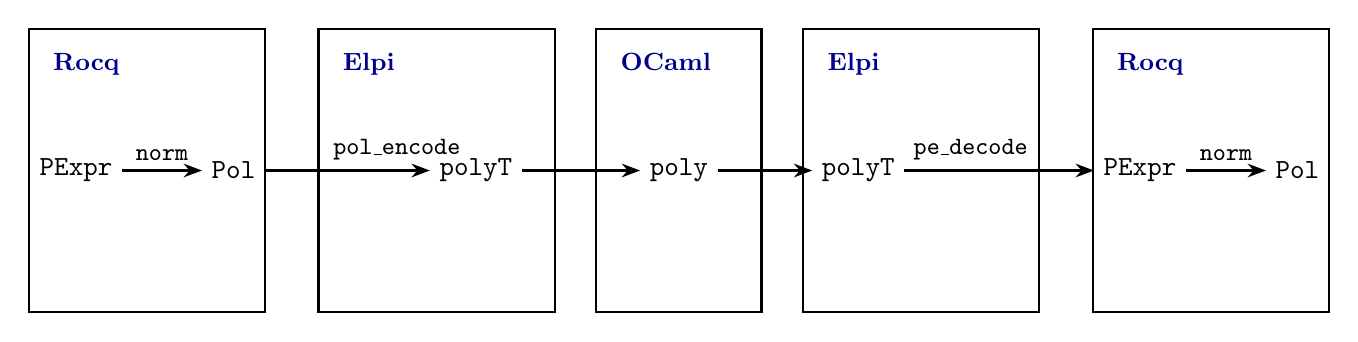
\begin{tikzpicture}[
    >=Stealth,
    stage/.style={
        draw,
        line width=0.8pt,
        minimum height=3.6cm,
        align=center
    },
    flow/.style={->, line width=0.8pt},
    label/.style={font=\small},
    stagetitle/.style={
    font=\bfseries\small,
    text=blue!55!black
}
]

\node[stage, minimum width=3.0cm] (rocq) {};
\node[anchor=north west, stagetitle] at ([xshift=2mm,yshift=-2mm]rocq.north west)
    {Rocq};

\node[stage, right=0.65cm of rocq,
      minimum width=3.0cm] (elpi1) {};
\node[anchor=north west, stagetitle] at ([xshift=2mm,yshift=-2mm]elpi1.north west)
    {Elpi};

\node[stage, right=0.5cm of elpi1,
      minimum width=2.1cm] (ocaml) {};
\node[anchor=north west, stagetitle] at ([xshift=2mm,yshift=-2mm]ocaml.north west)
    {OCaml};

\node[stage, right=0.5cm of ocaml,
      minimum width=3.0cm] (elpi2) {};
\node[anchor=north west, stagetitle] at ([xshift=2mm,yshift=-2mm]elpi2.north west)
    {Elpi};

\node (expr) at ([xshift=-0.9cm]rocq.center)
    {$\texttt{PExpr}$};

\node (pol) at ([xshift=1.1cm]rocq.center)
    {$\texttt{Pol}$};

\draw[flow] (expr) -- node[above,label] {\texttt{norm}} (pol);

\node (polyT1) at ([xshift=0.5cm]elpi1.center)
    {$\texttt{polyT}$};

\draw[flow] (pol.east) --
    node[above,label, pos=0.8] {\texttt{pol\_encode}}
    ([xshift=0cm]polyT1.west |- pol.east);

\node (poly)at (ocaml.center) {\texttt{poly}};

\draw[flow] (polyT1.east) --
    ( poly.west);

\node (polyT2) at ([xshift=-0.8cm]elpi2.center) {\texttt{polyT}};

\draw[flow] (poly.east) -- (polyT2.west);

\node[stage, minimum width=3.0cm, right=0.65cm of elpi2,] (rocq2) {};
\node[anchor=north west, stagetitle] at ([xshift=2mm,yshift=-2mm]rocq2.north west)
    {Rocq};

\node (expr2) at ([xshift=-0.9cm]rocq2.center)
    {$\texttt{PExpr}$};

\node (pol2) at ([xshift=1.1cm]rocq2.center)
    {$\texttt{Pol}$};
  \draw[flow] (polyT2.east) --
    node[above,label, pos=0.35] {\texttt{pe\_decode}}
    ([xshift=0cm]expr2.west |- polyT2.east);
\draw[flow] (expr2) -- node[above,label] {\texttt{norm}} (pol2);

\end{tikzpicture}
ELPI is a Prolog-like language for term manipulation
\cite{DBLP:conf/lpar/DunchevGCT15}. The integration of ELPI with Rocq builds on work on implementing
type theory in higher-order constraint logic programming
\cite{DBLP:conf/itp/Tassi19}. Its foreign-function interface is implemented in OCaml and connects ELPI to OCaml code loaded by the Rocq plugin.

To establish the correspondence between the type \texttt{polyT} (in ELPI) and the type \texttt{poly} (in OCaml) we only need to write some systematic code
that makes it explicit that some symbols in ELPI are connected to some
constructors in OCaml, for instance \texttt{add} symbol in ELPI is connected to
the \texttt{Add} constructor in OCaml, the types of both its arguments are
the same as the type produced by \texttt{add}, and pattern matching on a term
with the \texttt{Add} constructor is the same as inspecting the subterms of
a \texttt{add} term.  This correspondence is expressed by the following piece of
code (looking only at the description for \texttt{add}).
\label{sec:foreign-declaration}
\begin{lstlisting}[language=ML]
K("add", "binary addition", S(S(N)),
  B (fun x y -> Add (x, y)),
  M (fun ~ok ~ko t ->
    match t with Add (x, y) -> ok x y | _ -> ko ()))
\end{lstlisting}
Here the \texttt{K} expresses that we are describing a constructor correspondence.
The text \texttt{S (S (N))} expresses that \texttt{add} has two arguments, both of which are in the type currently being described.  Line 2 shows how to build a term
in OCaml corresponding to a term in ELPI whose head symbol is \texttt{add}.  This
line is especially useful when translating terms from ELPI to OCaml.
Conversely, lines 3 and 4 describe how to convert data from OCaml to ELPI.

This description for \texttt{add} is combined with descriptions for \texttt{mul},
\texttt{var} (for variables), and \texttt{pcst} (for constants) in a declaration
whose processing generates at the same time type declarations to be loaded
in ELPI and OCaml code that will perform the conversions when needed.

Similarly, the oracle's main function must be exposed as an
ELPI function.  In OCaml, this function is provided with type:
\begin{center}
  \texttt{Gcd.poly\_gcd : poly -> poly -> (int * poly * poly * poly)}.
\end{center}
The foreign function interface lets us declare a predicate \texttt{gcd\_poly} in
ELPI, where different parts of the result appear as different arguments of
the predicate.

When processing the declaration of \texttt{polyT} and \texttt{gcd\_poly}, the
foreign function tool produces the following declarations to be loaded
in ELPI.
\begin{lstlisting}
external symbol pcst : int -> polyT = "1".  % constant polynomial
external symbol var : int -> polyT = "1".  % indexed variable
external symbol add : polyT -> polyT -> polyT = "1".  % binary addition
external symbol mul : polyT -> polyT -> polyT = "1".  % binary multiplication

% [gcd_poly p1 p2 factor gcd p1_div p2_div] gcd is the greatest common
% divisor of polynomials p1 and p2, up to an integer factor 
%  p1_div is (factor * p1)/gcd, p2_div is (factor * p2)/gcd
external func gcd_poly polyT, polyT -> int, polyT, polyT, polyT.
\end{lstlisting}
It also produces some OCaml code that can be loaded in Rocq at the same time
as the oracle implementation.  With all this, any call to the ELPI
function \texttt{gcd\_poly} with two inputs of type \texttt{polyT} triggers
a call to \texttt{Gcd.poly\_gcd} in OCaml, with the two corresponding inputs
of type \texttt{poly}.  The results of this execution are then converted back
to type \texttt{polyT}.

The main justification theorem requires the various polynomials to be in
type \texttt{Pol}, but the ELPI function \texttt{gcd\_poly} returns values in
type \texttt{polyT}.  The easiest way to meet this requirement is to translate each term of type \texttt{polyT} into the corresponding term of type \texttt{PExpr}.  This
is easy because the type \texttt{polyT} is isomorphic to a sub-language of
\texttt{PExpr}.  The value of type \texttt{Pol} can then be obtained by calling
again the \texttt{norm} function.

The function \texttt{gcd\_poly} has inputs and outputs in types \texttt{polyT} and
\texttt{int}.  In the end we wrap this function into an ELPI function that takes
as inputs terms of the Rocq language, representing these polynomials and
numbers.  This is done with the following fragments of code:

\begin{lstlisting}
func pol_decode polyT -> term.
pol_decode PolyT_a Result :-
  pe_decode PolyT_a Pe_a,
  coq.reduction.vm.norm {{norm lp:Pe_a}} {{Pol Z}} Result.

func gcd_and_factors term, term -> term, term, term, term.
gcd_and_factors N D Ne De Gcd MZ :-
  pol_encode N Nx, pol_encode D Dx,
  gcd_poly Nx Dx M G N' D',
  pol_decode N' Ne, pol_decode D' De,
  pol_decode G Gcd, z_decode M MZ.
\end{lstlisting}
Note that in this code fragment, line 4 corresponds to the execution
of the function \texttt{norm}, which is actually written in the Gallina
language of the Rocq prover.

In turn, the computation can be made available to the \texttt{Ltac}
language in which
the \texttt{ring}-like tactics have been programmed.
\begin{lstlisting}
Elpi Tactic factorize_by_gcd.
Elpi Accumulate Plugin "ext.elpi".
Elpi Accumulate File encode.
Elpi Accumulate lp:{{

solve (goal _ _ _ _ [trm N, trm D] as G) GL :-
  gcd_and_factors N D N' D' Gcd LCM,
  (refine {{(lp:LCM, (lp:N', (lp:D', lp:Gcd)))}} G GL).
}}.
\end{lstlisting}
This describes how a piece of ELPI code can be viewed in Ltac as a Ltac function
that returns a value (in this case a Rocq quadruplet).  To call this function,
it will be necessary to write \texttt{elpi factorize\_by\_gcd N D}.

\subsection{Combining the oracle with the extended theorem}
We can now come back closer to the Rocq prover, where we only need to
finish programming our Ltac tactic that uses the result of the oracle in
combination with the extended theorem \texttt{Field\_rw\_pow\_correct\_w\_gcd}
(also described in Section~\ref{sec:extension-lemma}).
The main code is in Ltac, but the call to the oracle relies on a function
that was written in
ELPI.

For each of the formulas that we want to process with \texttt{field\_simplify},
the formula has already been reified, the numerator and denominator
have already been normalized (as ring formulas), and the theorem has already
been instantiated with this reified formula.  The tactic
\texttt{fraction\_finisher} is then called with the initial formula
(in variable \texttt{Term}), the instantiated theorem (in variable \texttt{hyp}),
the denominator (in variable \texttt{D}) and the numerator (in variable \texttt{N}).
The tactic performs the following actions:
\begin{lstlisting}
Ltac fraction_finisher Term hyp D N :=
let hyp2 := fresh "rew_l2" in
let res :=
  constr:(ltac:(elpi factorize_by_gcd ltac_term:(N) ltac_term:(D))) in
let F := eval cbv [fst] in (fst res) in
let N2 := eval cbv [fst snd] in (fst (snd res)) in
let D2 := eval cbv [fst snd] in (fst (snd (snd res))) in
let Gcd := eval cbv [snd fst] in (snd (snd (snd res))) in
assert (hyp2 := hyp F N2 D2 Gcd);
lazymatch type of hyp2 with
| _ -> _ -> _ -> _ -> ?t = ?r =>
change t with Term in hyp2;
  (try rewrite hyp2; clear hyp hyp2);
  [reduce_Pphi_pow | easy| easy | easy| reduce_PCond]
end.
\end{lstlisting}
At line 4, the oracle is called and the result stored in variable
\texttt{res}.  In lines 5 to 8 the various parts are retrieved, and at
line 9, the theorem is further instantiated with these parts.

After this instantiation the theorem statement
has the shape of an equality that is
valid solely under 4 assumptions (this is checked on lines 10-11).  The first
assumption is that the
number \(m\) is non-zero.  The next two assumptions are the factorization
identities, the last assumption is the collection of non-zero conditions
that was collected at the time of reification.

On line 12, we change the left-hand side
of the equality with the initial formula, because it is convertible
when reification is correct, then we rewrite with this conditional
equality, thus obtaining 5 goals.  The first one is where we performed
the rewriting operation, in this goal all polynomial normalization operations
should be performed (tactic \texttt{reduce\_Pphi\_pow} on line 14).  The next
three goals
should be trivially provable if the oracle performed its job correctly, hence
the three calls to the tactic \texttt{easy} on line 14.  We have no way to make
sure that the last goal can be proved automatically, but the formula
should be cleaned up so all functions coming from the \texttt{field}
infrastructure are reduced (tactic \texttt{reduce\_PCond} on line 14).

We defined a new tactic named \texttt{field\_simplify'} that integrates this
gcd computation.  We did not prove it, and this is not required to guarantee
the validity of the \texttt{field\_simplify'} tactic, but we believe that
this tactic essentially performs field normalization, while the original
\texttt{field\_simplify} tactic was not.

\subsection{A few examples}

Given a goal statement of the following form, 
\begin{lstlisting}
cos (2 * PI / 4) = cos (3 * PI / 6)
\end{lstlisting}
The previous tactic \texttt{field\_simplify (2 * PI / 4)} does not change
the goal.  On the other hand, our new tactic
\texttt{field\_simplify' (2 * PI / 4)} does replace \texttt{(2 * PI / 4)}
with \texttt{(PI / 2)}.

\subsection{Integrating in a deep behavior}
As a final result, we wish to have a simple tactic with no arguments that
solves the goals presented in our motivation.  We implemented such a tactic
by collecting all formulas that could potentially be improved using
\texttt{field\_simplify'} and repeating the process until the main goal
stabilizes. This is essentially the same computation as described in
Section~\ref{sec:deep-ring}.

We share code between \texttt{deep\_ring} and \texttt{deep\_field}.  The prefix
\texttt{deep} is here to express that ring or field normalization will occur, even
if the processed formulas are buried deeply inside arguments of functions outside
the corresponding languages.

The first stage is to collect all subformulas that are potential arguments
to \texttt{ring\_simplify} or \texttt{field\_simplify'}, and then call the simplify
tactics on these arguments.  After the first round, more normalization may
become apparent, and the process should be repeated until the formulas
stabilize.
\section{Quantitative evaluation}

To evaluate the computational cost of the approach, we consider a
family of increasingly nested expressions defined by the following
recursive functions:

\begin{lstlisting}[language=Rocq]
Fixpoint r (n : nat) (x : R) : R :=
  match n with
  | O => x
  | S n' => sin ((2*x - 2)* r n' x /2)
  end.

Fixpoint r_alt (n : nat) (x : R) : R :=
  match n with
  | O => x
  | S n' => sin ((x^2 - 1) * r_alt n' x / (x + 1))
  end.
\end{lstlisting}

For each depth $n$, we prove the following proposition
\begin{lstlisting}[language=Rocq]
forall x : R, forall p : x + 1 <> 0,
  r n x = r_alt n x.
\end{lstlisting}
The proof unfolds both recursive definitions, applies
\texttt{deep\_field}, and finishes with \texttt{reflexivity} and \texttt{nra} to get rid of side conditions.
The experiment therefore measures the cost of simplifying algebraic
expressions nested inside successive applications of $\sin$.

The benchmark measures both the tactic execution time and the total wall-clock time. The former is obtained using Rocq's \texttt{Time} command, whereas the latter includes the overhead of processing and compiling the surrounding proof.

\begin{figure}[htbp]
  \centering
  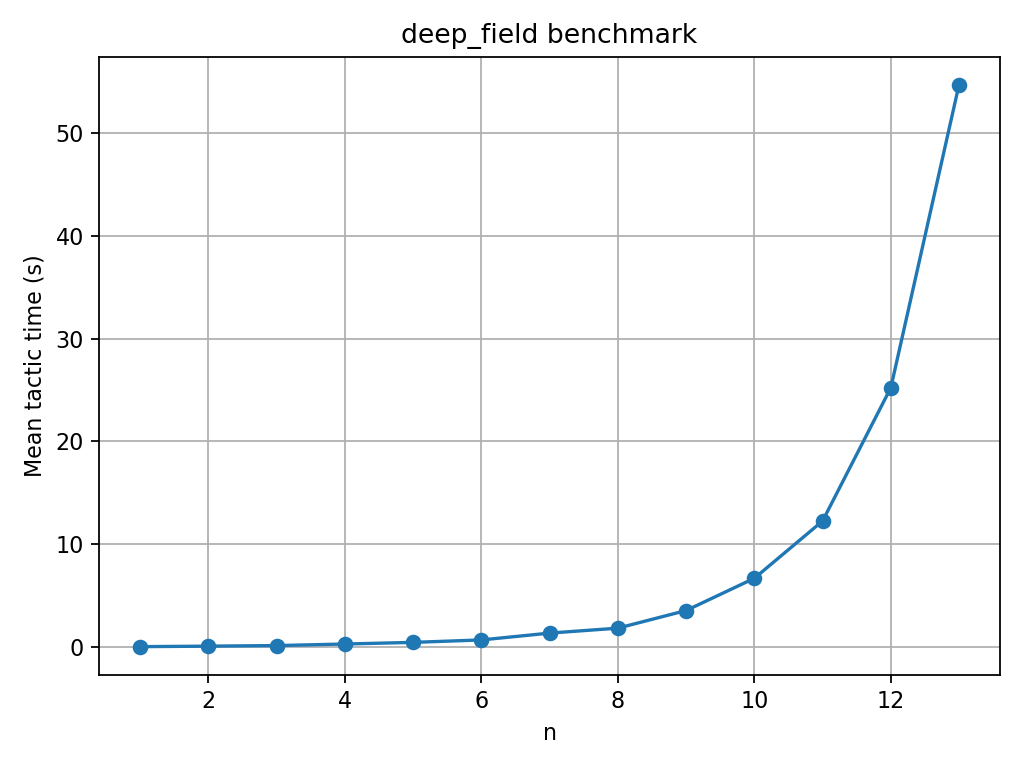
\includegraphics[width=0.8\textwidth]{images/benchmark.png}
  \caption{Measured execution times as a function of nesting depth $n$.}
  \label{fig:execution-times}
\end{figure}
We evaluated 13 instances, for $(1 \leq n \leq 13)$, running each instance 10 times and reporting the mean execution time. The mean tactic execution time increased from 0.038 seconds at n=1 to 54.715 seconds at n=13, while the mean wall-clock time increased from 0.499 seconds to 74.090 seconds.

The execution time increases rapidly with the nesting depth. However, the practical relevance of this growth depends on the depths encountered in actual proofs. Undergraduate students are unlikely to encounter formulas with a nesting depth greater than, say, 5, so the cost is acceptable.




% The experiment also highlights an important difference between deep ring and
% deep field simplification. For ring expressions, normalization naturally
% provides a canonical polynomial representation, so recursively simplifying
% function arguments is sufficient to make equivalent terms syntactically
% equal. For field expressions, equality can instead be established by cross
% multiplication without producing such a common representation. The gcd
% computation addresses this additional representation problem by making it possible to reduce the fraction.

% The current extension nevertheless operates at a limited point in the field
% simplification process. It handles the field expression selected by the
% existing field-simplification infrastructure, but it does not yet recursively
% traverse arbitrary nested field expressions in the same way as the deep ring
% procedure. A fully general deep field simplification procedure would therefore
% require extending the recursive traversal.

% \section{Future work}

% Several extensions remain possible:

% \begin{itemize}
% \item extending the gcd-based reduction to a general deep field
% simplification procedure;
% \item improving the staging of normalization and rewriting to avoid
% unnecessary computation;
% \item reducing the number of generated proof obligations;
% \item extending deep ring and field reasoning to expressions involving
% exponents;
% \item exploring similar techniques for commutative-group isomorphisms;
% \item strengthening the polynomial gcd computation to support a broader
% range of integer representations.
% \end{itemize}


\section{Conclusion}


Extending reflexive algebraic tactics to expressions occurring inside
unrecognized function applications requires more than recursively invoking
the existing normalization procedures. For ring expressions, polynomial
normalization already provides a canonical representation that can be
propagated through the surrounding function application. For field expressions, the use of cross multiplication means that reducing each expression to a normal form is not necessary. As a result, no tactic was
provided to perform field normalization.  Despite the similarity in their names,
\texttt{field\_simplify} does not provide what \texttt{ring\_simplify} does.

This work uses a polynomial gcd computation to provide the missing
normalization. An
OCaml oracle computes the common factor and the corresponding numerator and
denominator quotients, while Rocq verifies the resulting factorization
identities and side conditions. ELPI provides the interface between the
external computation and the existing Ltac and field-simplification
infrastructure.

It should be noted that a formally verified implementation of Buchberger's
algorithm was studied by L. Théry \cite{thery2001machine}.  When consulted
about implementing the algorithm for this need, he nevertheless recommended using an untrusted implementation.

The current implementation is a proof-of-concept, implemented using the
simplest form of bridge between Rocq code and the external oracle.  There
are several directions in which to progress.  The first pass is to
reconsider all data transformations to reduce the number of intermediate
steps.  In particular, we think that translating directly the \texttt{Pol} type from
Rocq into the \texttt{mpoly} type from OCaml and back, without going through the
\texttt{poly}, \texttt{polyT}, and \texttt{PExpr}, and without needing to execute
the Rocq-defined \texttt{norm} function.

A second area of progress is to choose carefully the order in which
sub-expressions are considered for field or ring normalization.  The leading
idea is that expressions should not be considered for normalization
if they still contain function calls with subterms that have not been
normalized yet.  This should lead to a
procedure that processes nested expressions from
the inside out. This could also reduce unnecessary computation and the
number of generated side conditions, but its effectiveness must be
evaluated experimentally. Measurements of proof success, execution
time, and generated side conditions would help assess the practical
benefits of the approach.

The broader objective is to make algebraic automation behave more
naturally on mathematical expressions, while preserving the
proof guarantees of Rocq. The combination of recursive
simplification, polynomial factorization, and automatically verifiable
normalization provides a foundation for pursuing this objective
beyond the ring and field fragments.

\paragraph{Acknowledgements}  The authors would like to thank Laurent Théry,
Davide Fissore, and Enrico Tassi for numerous suggestions and help on this
experiment.
\bibliographystyle{alpha-fr}

\bibliography{references}
\end{document}
